\section{Inference}
\label{inference}

An important contribution of \affe is its principal type inference.
We now formulate our inference algorithm
based on the $HM(X)$ framework~\citep{DBLP:journals/tapos/OderskySW99}.
$HM(X)$ is a Hindley-Milner type system for a language
with qualified types where constraints are expressed in an arbitrary
theory $X$.
Most importantly,
$HM(X)$ ensures principal type inference
when $X$ respects the specified properties.
We apply HM(X) to a concrete constraint language which we name $\CL$.
We adapt and extend HM(X)'s existing rules to support kind inference,
track linearity and handle borrows and regions. Finally, we
formulate an appropriate constraint solving algorithm for $\CL$
which solves and simplifies constraints in a principled way.
We start by various preliminary definitions.

\subsection{Preliminaries}

Unlike the syntax-directed version of our type system, knowing which elements
are input and output or our inference judgements is critical. In the rest
of this section, when presenting a new judgement,
we write input parameters in \textbf{\textcolor{DarkSlateBlue}{bold blue}}. The rest will then be
output parameters.

\paragraph{Usage environments}

% One novelty of our inference  judgement now
% returns a type environment, which we call ``usage environment'' and commonly
% write $\Sv$, to summarize how variables and borrows are used inside
% the expression.

In order to determine if a variable is used in an affine manner, we must track
its uses and the associated kinds. For instance, in the expression
$(x,x)$, $x$ is used twice. If $x$ is of type $\tau$, which is of kind $k$,
we must add the constraint $\Cleq{k}{\kun}$.
%
In order to infer such constraints, our inference judgement will not only
take an environment as parameter but also return an environment which
we call ``usage environment'' and which summarizes how variables and borrows
are used. Usage environments follow the exact same grammar
as normal environments. In order to distinguish them more easily,
we denote them by $\Sv$.

In \cref{sdtyping}, we used relations to split environments in two and to
transform suspended bindings into borrows inside a region.
These relations take as argument a constraint which validates
the transformations.
In the context of inference, we define new judgements which \emph{infer}
the constraints.
\begin{itemize}[leftmargin=*]
\item $\bsplit{C}{\Sv}{\inP{\Sv_1}}{\inP{\Sv_2}}$.
  Given two usage environments $\inP{\Sv_1}$ and $\inP{\Sv_2}$
  (inferred from two subexpressions, for instance),
  we return $\Sv$, the merged environment, and $C$, a set
  of constraints that must be respected.
  This relation is total and non-ambiguous given $\Sv_1$ and $\Sv_2$
  and uses the same rules as the one presented in \cref{sdtyping:split}.
\item $\bregion[\inP{n}]{C}{\inP{x}}{\Sv}{\inP\Sv'}$.
  Given a usage environment $\inP{\Sv'}$, a nesting level $\inP{n}$,
  and a variable name $\inP{x}$, we return
  $\Sv$ where the borrow binding of $x$ in $\Sv'$, if it exists,
  is replaced by
  a suspended binding. We also return $C$, a set of constraints that must
  be respected.
  Again, the relation is total and non-ambiguous for any given $\Sv'$,
  $n$ and $x$,
  and uses the rules presented in \cref{sdtyping:regions}.
\end{itemize}

The relations used for syntax-directed typing can trivially be defined
in terms of these new relations by using constraint entailment.
All relations are fully described in \cref{typ:extra:envs}.

\paragraph{Constraint normalization}

The HM(X) framework assumes the existence of a ``$\operatorname{normalize}$''
function which takes a constraint $C$, a substitution $\psi$ and returns a
simplified constraint $C'$
and an updated substitution $\unif'$.
Normalization must return a normal form such that $\unif'$ is a most general unifier.
We detail the implementation
of the normalization function and its property in \cref{infer:solving}.
In the meantime, we simply
assume the existence of such a function for our constraint system.

\subsection{Type inference}

We write $\inferW{\Sv}{(C,\unif)}{\inP{\E}}{\inP{e}}{\tau}$ when
$\inP{e}$\ has type $\tau$ in $\inP{\E}$ under the constraints $C$ and unifier $\unif$
with a usage environment $\Sv$. $\inP\E$ and $\inP{e}$ are the input parameters of our
inference algorithm.
Unlike in the syntax-directed version, $\E$ only regular and type bindings.
Suspended and borrow bindings can only be present in $\Sv$.
We revisit some of the syntax-directed rules presented in \cref{sdtyping}
to highlight the novelties
of our inference algorithm and the differences with the syntax-directed
system.
The complete type inference rules are shown in \cref{appendix:infer}.

\subsubsection{Environments and bindings}
\label{infer:envs}
%
\begin{figure*}[tb]
  \begin{mathpar}
    \ruleIVar
    \and
    \ruleIAbs
    \and
    % \ruleILet
    % \hfill
    \ruleIRegion
    \and
    \ruleIPair
    \and
    \inferrule{}
    { \Weaken_{\bvar{x}{\sigma}}(\Sv) =
      \text{if } (x\in\Sv) \text{ then} \Ctrue \text{else }
      \Cleq{\sigma}{\kaff_\infty}
      % \begin{dcases}
      %   \Ctrue&\text{if } x\in\Sv\\
      %   \Cleq{\sigma}{\kaff_\infty}&\\
      % \end{dcases}
      % \\\\\\
      % \generalize{C}{\E}{\tau} =
      % (\Cproj{(\Multi{\kvar},\Multi{\tvar})}{C},
      % \forall (\Multi{\kvar},\Multi{\tvar}).\qual{C}{\tau})\\
      % \text{ where}\\\\
      % \Multi{\kvar},\Multi{\tvar} = (\fv{\tau}\cup\fv{C})\setminus\fv{\E}
    }
  \end{mathpar}
  \vspace{-15pt}
  \caption{Selected inference rules -- $\inferW{\Sv}{(C,\unif)}{\inP{\E}}{\inP{e}}{\tau}$}
  \label{rule:infer:envs}
  \label{rule:infer:envrules}
  \label{rule:infer:let}
\end{figure*}
%
In our syntax-directed system, we ensured
that linear variables are not discarded at the \emph{leaves}, through
the {\sc Var} rule. In the inference algorithm, we operate in the opposite
direction: we collect data from the leaves, and only enforce linearity
at \emph{binders}. This is reflected in the {\sc Var$_I$} and
{\sc Abs$_I$} rules presented in \cref{rule:infer:envs}.
Typing for variables is very similar to traditional (non-affine) ML
typing. The only difference is that we collect
the fact that $x$ was used with the scheme $\schm$ by returning
a usage environment $\Sv = \{ \bvar{x}{\schm} \}$.
%
This usage environment is in turn used at each binder to enforce proper
usage of linear variable via the $\Weaken$ property.
We demonstrate how this is achieved for lambda expressions
in the {\sc Abs$_I$} rule.
First, we typecheck the body of the lambda and obtain a usage
environment $\Sv_x$. Just like in the syntax-directed type system,
we introduce the constraint
$\Cleq{\Sv\Sdel{x}}{\kvar}$ which properly accounts for captures in
the body of the lambda expression. We also introduce the constraint
$\Weaken_{\bvar{x}{\sigma}}(\Sv)$, which is false only if weakening
is necessary but impossible due to linearity.
The $\Weaken$ constraint is introduced at each binding point in the program
such as let-bindings and pattern matching.

Finally, we use normalization on complex constraints to ensure
that the inference algorithm always return the simplest possible
constraints and unifiers.



\subsubsection{Splitting and Regions}
\label{infer:split}
\label{infer:regions}

The inference version
of the {\sc Pair} and {\sc Region} rules is shown in \cref{rule:infer:envrules}.
While the rules are quite similar to the original version, the usage
environment $\Sv$ is now an \emph{output} of the algorithm.
As such, we use the ``inference'' version of the relations on
the environment,
$\bsplit{C}{\Sv}{\inP{\Sv_1}}{\inP{\Sv_2}}$
and $\bregion{C}{\inP{x}}{\Sv}{\inP\Sv'}$,
which returns the necessary constraints.
As appropriate for inference, these relations
are total and non ambiguous for their input parameters ($\Sv_1, \Sv_2$ and $\Sv'$, respectively).
We then collect all constraints and normalize them.



\subsection{Constraint solving}
\label{infer:solving}



\newcommand\A{\mathcal A}
\newcommand\SC{\mathcal S}



%
% \begin{figure}[tb]
%   \centering
%   \begin{align*}
%     C &::= \Cleq{\tau_1}{\tau_2}
%         \mid \Cleq{k_1}{k_2}
%         \mid C_1 \Cand C_2
%         \mid \Cproj{\tvar}{C}
%         \mid \Cproj{\kvar}{C}
%   \end{align*}
%   \caption{The constraint language}
%   \label{grammar:constraint}
%   % \begin{minipage}{0.65\linewidth}
  \begin{mathpar}
    \inferrule[Lat-UAL]{}{\kun \lk \kaff \lk \klin}
    \and
    \inferrule[Lat-Level]{\mul \lk \mul' \and n \lk n'}{\mul_n \lk_\Lat \mul'_{n'}}
  \end{mathpar}
\end{minipage}~
\begin{minipage}{0.2\linewidth}
  \centering
  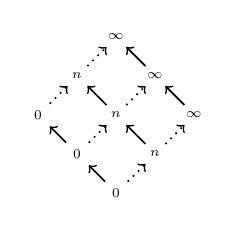
\begin{tikzpicture}
    [->,auto,semithick, every node/.style={scale=0.7}]
    \node(U) {$\kun_0$} ;
    \node(A) [above left of=U] {$\kaff_0$} ;
    \node(L) [above left of=A] {$\klin_0$} ;
    \node(Un) [above right of=U] {$\kun_n$} ;
    \node(An) [above left of=Un] {$\kaff_n$} ;
    \node(Ln) [above left of=An] {$\klin_n$} ;
    \node(Uinf) [above right of=Un] {$\kun_\infty$} ;
    \node(Ainf) [above left of=Uinf] {$\kaff_\infty$} ;
    \node(Linf) [above left of=Ainf] {$\klin_\infty$} ;
    \path
    (U) edge (A)
    (A) edge (L)
    (Un) edge (An)
    (An) edge (Ln)
    (Uinf) edge (Ainf)
    (Ainf) edge (Linf)
    ;
    \path[dotted]
    (U) edge (Un)
    (A) edge (An)
    (L) edge (Ln)
    (Un) edge (Uinf)
    (An) edge (Ainf)
    (Ln) edge (Linf)
    ;
  \end{tikzpicture}
\end{minipage}

%%% Local Variables:
%%% mode: latex
%%% TeX-master: "../main"
%%% End:

%   % \caption{Lattice inequalities -- $k \lk_\Lat k'$}
%   \begin{mathpar}
  \inferrule
  {}{ \entail{}{\Cleq{\kvar}{\kaff}} }
  \and
  \inferrule
  {}{ \entail{}{\Cleq{\kun}{\kvar}} }
  \and
  \inferrule
  {}{ \entail{}{\Cleq{\kvar}{\kvar}} }
  \and
  % \inferrule
  % {\Cleq{k}{k'} \in C}{ \entail{C}{\Cleq{k}{k'}} }
  % \and
  % \inferrule
  % { \entail{C}{\Cleq{x_1}{x}}\\
  %   \entail{C}{\Cleq{x}{x_2}}
  % }
  % { \entail{C}{\Cleq{x_1}{x_2}} }
  % \and
  % \inferrule
  % { \entail{C}{D} }
  % { \entail{C}{\Cproj{x}{D}} }
  % \\
  \inferrule
  { \entail{C}{\Cleq{\tau'_1}{\tau_1}}\\
    \entail{C}{\Cleq{\tau_2}{\tau'_2}}\\
    \entail{C}{\Cleq{k}{k'}}
  }
  { \entail{C}{\Cleq{\tau_1\tarr{k}\tau_2}{\tau'_1\tarr{k'}\tau'_2}} }
  \and
  \inferrule
  { \forall i,\ \entail{C}{\Cleq{\tau_i}{\tau_i}}\\
  }
  { \entail{C}{\Cleq{\tapp{t}{(\tau_i)}}{\tapp{t}{(\tau'_i)}}} }
  \and
  
  % \and
  % \inferrule
  % { \entail{C}{\Cleq{k}{k'}} \\
  %   \entail{C}{\Cleq{k'}{k}} }
  % { \entail{C}{\Ceq{k}{k'}} }
  % \and
  % \inferrule
  % { \entail{C}{\Cleq{k}{k'}} }
  % { \entail{C}{\Ckind{\tau_0\tarr{k}\tau_1}}{k'}}
  % \and
  % \text{Completion to form a cylindric constraint system.}
\end{mathpar}

%%% Local Variables:
%%% mode: latex
%%% TeX-master: "../main"
%%% End:

%   \caption{Base entailment rules -- $\entail{\inP{C}}{\inP{D}}$ }
%   \label{rules:entail}
% \end{figure}



For concision, we demonstrate our constraint solving
algorithm on an example. The complete constraint system is
defined in \cref{appendix:constraints}.
%
\label{solving:example}

\begin{figure}[tbp]
  \centering
  \begin{tikzpicture}[node distance=6mm,xscale=1.2,yscale=0.7,.every edge/.style=[link,->,>=latex,thick]]
    \node (U) {$\kun$} ;
    \node[above left=of U] (x) {$\kvar_x$} ;
    \node[above=of x] (r) {$\kvar_r$};
    \node[left=of x] (g) {$\kvar_\gamma$} ;
    \node[right=of x] (b) {$\kvar_\beta$} ;
    \node[right=of b] (3) {$\kvar_3$} ;
    \node[above=of 3] (f) {$\kvar_f$} ;
    \node[above=of f] (1) {$\kvar_1$} ;

    \draw (x) to[bend right] (U) ;
    \draw (x) -> (r) ;
    \draw (b) -> (r) ;
    \draw (g) -> (x) ;
    \draw (3) -> (f) ;
    \draw (f) -> (1) ;

    \draw[blue] (3) to[bend right] (1);

    \node at (-0.5,-0.5) {Before};
    
    \begin{scope}[dashed,gray]
      \draw (U) to[bend right] (x) ;
      \draw (U) to (b) ;
      \draw (U) to[bend left] (g) ;
      \draw (U) to (r) ;
      \draw (U) to (1) ;
      \draw (U) to (3) ;
      \draw (U) to (f) ;
    \end{scope}
  
    \begin{scope}[on background layer]
      \node[fill=green!20,draw=green,
      inner sep=-1pt,ellipse,rotate fit=-20,fit=(U.south) (x) (g)] {};
      \node[fill=red!20,draw=red, inner sep=-2pt, circle,fit=(r)] {};
      \node[fill=red!20,draw=red, inner sep=-2pt, circle,fit=(f)] {};
    \end{scope}
  \end{tikzpicture}~
  \vrule~
  \begin{tikzpicture}[node distance=7mm,every edge/.style=[link,->,>=latex,thick]]
    \node (b) {$\kvar_\beta$} ;
    \node[right=of b] (3) {$\kvar_3$} ;
    \node[above=of 3] (f) {} ;
    \node[above=of f] (1) {$\kvar_1$} ;

    \draw (3) to[bend right] (1);

    \node at (0.5,-1.5) {After};
  \end{tikzpicture}
  \vspace{-5pt}
    \caption{Graph representing the example constraints}
    \label{example:graph}
    % \caption{Final state of the graph}
    \label{example:graph:final}
\end{figure}

Consider the expression $\lam{f}{\lam{x}{(\app{f}{x},x)}}$.
The inference algorithm yields the following constraints:
%
\begin{align*}
  \E &= (\tvar_f : \kvar_f)
  (\tvar_x : \kvar_x)\dots\\
  C &= (\tvar_f \leq \gamma \tarr{\kvar_1} \beta )
  \Cand
  (\gamma \leq \tvar_x)
  \Cand
  (\beta \times  \tvar_x \leq \alpha_r)
  \Cand
  (\kvar_x \leq \kun)
\end{align*}

The first step of the algorithm uses Herbrand unification to obtain
a type skeleton. 
$$
(\gamma \tarr{\kvar_3} \beta) \tarr{\kvar_2} \gamma \tarr{\kvar_1} \beta \times  \gamma$$

In addition, we obtain the following kind constraints: 
\[\begin{aligned}
    % \Cproj{\kvar_r}\Cproj{\kvar_f}\Cproj{\kvar_x}{}
    &(\kvar_x \leq \kun)
    \Cand
    (\kvar_\gamma \leq \kvar_x)
    \Cand
    (\kvar_x \leq \kvar_r)
    \Cand
    (\kvar_\beta \leq \kvar_r)
    \Cand
    (\kvar_3 \leq \kvar_f)
    \Cand
    (\kvar_f \leq \kvar_1)
\end{aligned}\]
% Since $\kvar_r$, $\kvar_f$ and $\kvar_x$ are not present in the type skeleton,
% they are existentially quantified.

We translate these constraints into a relation whose graph
is shown in \cref{example:graph}.
%
The algorithm then proceeds as follow:
\begin{itemize}[noitemsep]
\item From the constraints above, we deduce the graph shown
  with plain arrows on the left of \cref{example:graph}.
\item We add all the dashed arrows by saturating
  lattice inequalities. For clarity, we only show $\kun$.
\item We identify the connected component circled in
  {\color{ForestGreen} green}.
  We deduce $\kvar_\gamma = \kvar_x = \kun$.
\item We take the transitive closure, which adds the
  arrow in {\color{blue} blue} from $\kvar_3$ to $\kvar_1$.
\item We remove the remaining nodes not present in the type skeleton (colored in {\color{red} red}): $\kvar_r$ and $\kvar_f$.
\item We clean up the graph (transitive reduction, remove unneeded constants, \dots),
  and obtain the graph shown on the right.
  We deduce $\kvar_3 \leq \kvar_1$.
\end{itemize}

The final constraint is thus
$$\kvar_\gamma = \kvar_x = \kun \Cand \kvar_3 \leq \kvar_1$$
If we were to generalize, we would obtain the type scheme:
$$\forall \kvar_\beta \kvar_1 \kvar_2 \kvar_3
(\gamma : \kun) (\beta : \kvar_\beta).\ %
\qual
{\Cleq{\kvar_3}{\kvar_1}}
{(\gamma \tarr{\kvar_3} \beta) \tarr{\kvar_2} \gamma \tarr{\kvar_1} \beta \times  \gamma}$$

We can further simplify this type by exploiting variance. As $\kvar_1$
and $\kvar_2$ are only used in covariant position, they can be
replaced by their lower bounds, $\kvar_3$ and $\kun$. 
By removing the unused quantifiers, we obtain a much simplified equivalent type:
$$
\forall \kvar
(\gamma : \kun).
{(\gamma \tarr{\kvar} \beta) \tarr{} \gamma \tarr{\kvar} \beta \times  \gamma}$$



%%% Local Variables:
%%% mode: latex
%%% TeX-master: "../main"
%%% End:


Our algorithm respect the properties
of HM(X), computes principal normal forms
and simplifies constraints significantly.
All the simplification mechanisms presented
here, including the variance-based one, are complete.
It is also possible to add ``best-effort'' simplification
rules which help reduce the size of inferred signatures even further
\citep{DBLP:conf/aplas/Simonet03}.

% 
% We now show that this algorithm is well-behaved with respect to entailment
% and computes unique normal forms.

% \begin{property}[Principal normal form]
%   Normalization computes principal normal forms for $\CL$, i.e.
%   given a constraint $D\in\CL$, a substitution $\phi$ and
%   $(C,\unif) = \normalize{D}{\phi}$,
%   then $\phi\leq\unif$,
%   $C \equivC \unif D$ and
%   $\unif C = C$.
% \end{property}

% \begin{property}[Principal constraints]
%   $\CL$ has the principal constraint property, i.e.
%   for every $D\in\CL$, and a substitution $\unif$,
%   either $D$ does not have a normal form, or it has
%   a principal normal form.
% \end{property}

% \begin{property}[Regular constraint system]
%   $\CL$ is regular, ie, for $x, x'$ two types or kinds,
%   $\entail{}{\Ceq{x}{x'}}$ implies
%   $\fv{x} = \fv{x'}$
% \end{property}

% The proofs are given in \cref{appendix:constraints}. These three properties
% are sufficient to state that $HM(\CL)$ provides principal type inference.
% However, we use an extension of HM(X) with kind inference
% and affine types and borrows.
% We now show that HM(X)'s completeness and soundness theorems are still valid on
% this extended system.

\subsection{Soundness and Principality}

We now state that our extended inference algorithm still satisfies the soundness
and completeness properties of HM(X).
% This is achieved by extending
% the original proofs from HM(X), which is done in \cref{appendix:infer}.
%
The first theorem states that our inference algorithm is sound
with respect to the syntax-directed type system.

\begin{theorem}[Soundness of inference]
  Given a type environment $\E$ containing only value bindings,
  $\E|_\tau$ containing only type bindings, and a term $e$:\\
  if $\inferW{\Sv}{(C,\unif)}{\E;\E_\tau}{e}{\tau}$\\
  then $\inferS{C}{\unif(\Sv;\E_\tau)}{e}{\tau}$, $\unif C = C$ and $\unif \tau = \tau$
\end{theorem}

The syntax-directed derivation holds with the usage environment $\Sv$ instead of the originally provided environment $\E$. Indeed,
$\E$ does not contain suspended and borrow bindings, since those
are discovered on the fly and recorded in $\Sv$. The type binding, however,
are directly taken from the syntax-directed derivation.

The second theorem states that our algorithm is complete: for any given
syntax-directed typing derivation, our inference algorithm can find
a derivation that gives a type at least as general.
For this, we need first to provide a few additional definitions.

% \begin{definition}[More general unifier]
%   Given a set of variable $U$ and $\unif$, $\unif'$ and $\phi$
%   substitutions. \\
%   Then
%   $\unif \leq^{\phi}_{U} \unif'$ iff $(\phi \circ \unif)|_{U} = \unif'|_U$.
% \end{definition}

\begin{definition}[Instance relation]
  Given a constraint $C$ and two schemes
  $\schm = \forall \Multi\tvar. \qual{D}{\tau}$ and
  $\schm' = \forall \Multi\tvar'. \qual{D'}{\tau'} $.
  Then $\entail{C}{\schm \preceq \schm'}$
  iff $\entail{C}{\subst{\tvar}{\tau''} D}$
  and $\entail{C\Cand D'}{\Cleq{\subst{\tvar}{\tau''}\tau}{\tau'}}$
\end{definition}

\begin{definition}[Flattened Environment]
A flattened environment,
written as $\Eflat\E$, is the environment
where all the binders are replaced by normal ones. More formally:
\begin{align*}
  \Eflat\E
  =& \left\{\bvar{x}{\tau}\in\E \mid
    \vee \bvar{\borrow{x}}{\borrowty{k}{\tau}}\in\E
    \vee \svar{x}{\tau}^n\in\E
    \right\}\\
  &\cup \left\{ \bvar{\tvar}{k} \mid \bvar{\tvar}{k}\in\E \right\}
\end{align*}
\end{definition}


We can then state principality.

% \begin{theorem}[Completeness]
%   Given $\inferS{C'}{\E'}{e}{\tau'}$ and
%   $\entail{}{\unif'\E \preceq \E'}$.
%   Then $$\inferW{\Sv}{(C,\unif)}{\Eflat\E}{e}{\tau}$$
%   for some environment $\Sv$,
%   substitution $\unif$, constraint $C$ and type $\tau$ such
%   that
%   \begin{align*}
%     \unif &\leq^{\phi}_{\fv{\E}} \unif'
%     &\entail{C'&}{\phi C}
%     &\entail{&}{\phi \schm \preceq \schm'}
%     &\Sv&\subset\E
%     % &( C, \schm, \unif) &\leq (C',\schm',\unif')
%   \end{align*}
%   where $\schm' = \generalize{C'}{\E'}{\tau'}$
%   and $\schm = \generalize{C}{\E}{\tau}$
% \end{theorem}

% Finally, principality is a direct application of completeness to
% toplevel programs.

\begin{theorem}[Principality]
  Let $\inferS{\Ctrue}{\E}{e}{\schm}$ a closed typing judgement.\\
  Then $\inferW{\Sv}{(C,\unif)}{\Eflat\E}{e}{\tau}$
  such that:
  \begin{align*}
    (\Ctrue,\schm_o) &= \generalize{C}{\unif\E}{\tau}
    &\entail{&}{\schm_o \preceq \schm}
    % &( C, \schm, \unif) &\leq (C',\schm',\unif')
  \end{align*}


\end{theorem}

%%% Local Variables:
%%% mode: latex
%%% TeX-master: "../main"
%%% End:
